\documentclass[12pt]{article}
\usepackage{graphicx}
\usepackage{html}
\usepackage{lecture}
\usepackage{epstopdf}
\usepackage{url}

\newcommand{\copyrightYears}{2012-2017}

\title{Population genomics}

\begin{document}

\maketitle

\thispagestyle{first}

\section*{Introduction}

In the past decade, the development of high-throughput methods for
genomic sequencing (next-generation sequencing: NGS) have
revolutionized how many geneticists collect data. It is now possible
to produce so much data so rapidly that simply storing and processing
the data poses great challenges~\cite{Nekrutenko-Taylor-2012}. The
Nekrutenko and Taylor review~\cite{Nekrutenko-Taylor-2012} doesn't
even discuss the new challenges that face population geneticists and
evolutionary biologists as they start to take advantage of those
tools, nor did it discuss the promise these data hold for providing
new insight into long-standing questions, but the challenges and the
promise are at least as great as those they do
describe.\index{next-generation sequencing}

To some extent the most important opportunity provided by NGS
sequencing is simply that we now have a lot more data to answer the
same questions. For example, using a technique like RAD
sequencing~\cite{Baird-etal-2008} or genotyping-by-sequencing
(GBS:~\cite{Elshire-etal-2011}), it is now possible to identify
thousands of polymorphic SNP markers in non-model organisms, even if
you don't have a reference genome available. As we've seen several
times this semester, the variance associated with drift is
enormous. Many SNPs identified through RAD-Seq or GBS are likely to be
independently inherited. Thus, the amount and pattern of variation at
each locus will represent an independent sample from the underlying
evolutionary process. As a result, we should be able to get much
better estimates of fundamental parameters like $\theta=4N_e\mu$,
$M=4N_em$, and $R=4N_er$ and to have much greater power to
discriminate among different evolutionary scenarios. Willing et
al.~\cite{Willing-etal-2012}, for example, present simulations
suggesting that accurate estimates of $F_{ST}$ are possible with
sample sizes as small as 4--6 individuals per population, so long as
the number of markers used for inference is greater than
1000.\index{RAD sequencing}\index{next-generation sequencing!estimating $F_{ST}$}\index{genotyping-by-sequencing}

\section*{A quick overview of NGS methods}

I won't review the chemistry used for next-generation sequencing. It
changes very rapidly, and I can't keep up with it. Suffice it to say
that 454 Life Sciences, Illumina, PacBio, and probably other companies
I don't know about each have different approaches to very high
throughput DNA sequencing. What they all have in common is that the
whole genome is broken into small fragments and sequnced and that a
single run through the machine produces an enormous amount of data,
900-1800 Gb from a HiSeq X for
example~(\url{http://www.illumina.com/systems/sequencing.html};
accessed 26 April 2015).\footnote{In NGS applications for phylogeny, a
  strategy of targeted enrichment is often used. In this approach,
  pre-identified parts of the genome are ``baited'' using primers and
  those parts of the genome are enriched through PCR before the
  sequencing library is constructed~\cite{Lemmon-etal-2012}.} 

\subsection*{RAD sequencing}\index{RAD sequencing}

Baird et al.~\cite{Baird-etal-2008} introduced RAD almost 10 years
ago. One of its great attraction for evolutionary geneticists is that
RAD-seq can be used in any organism from which you can extract DNA and
the laboratory manipulations are relatively straightforward.

\begin{itemize}

\item Digest genomic DNA from each individual with a restriction
  enzyme, and ligate an adapter to the resulting fragments. The
  adapter includes a forward amplification primer, a sequencing primer
  and a ``barcode'' used to identify the individual from which the DNA
  was extracted.

\item Pool the individually barcoded samples~(``normalizing'' the
  mixture so that roughly equal amounts of DNA from each individual
  are present) shear them and select those of a size appropriate for
  the sequencing platform you are using.

\item Ligate a second adapter to the sample, where the second adapter
  is the reverse complement of the reverse amplification primer. 

\item PCR amplification will enrich only DNA fragments having both the
  forward and reverse amplification primer.

\end{itemize}

The resulting library consists of sequences within a relatively small
distance from restriction sites. 

\subsection*{Genotyping-by-sequencing}\index{genotyping-by-sequencing}

Genotyping-by-sequencing~(GBS) is a similar approach. 

\begin{itemize}

\item Digest genomic DNA with a restriction enzyme and ligate two
  adapters to the genomic fragments. One adapter contains a barcode
  and the other does not.

\item Pool the samples.

\item PCR amplify and sequence. Not all ligated fragments will be
  sequenced because some will contain only one adapter and some
  fragments will be too long for the NGS platform.

\end{itemize}

Once an investigator has her sequenced fragments back, she can either
map the fragments back to a reference genome or she can assemble the
fragments into orthologous sequences {\it de novo}. I'm not going to
discuss either of those processes, but you can imagine that there's a
lot of bioinformatic processing going on. What I want to focus on is
what you do with the data and how you interpret it.

\section*{Next-generation phylogeography}\index{next-generation sequencing!phylogeography}

The American pitcher plant mosquito {\it Wyeomyia
  smithii\/} has been extensively studied for many years. It's a model
organism for ecology, but its genome has not been sequenced. An
analysis of {\it COI} from 20 populatins and two outgroups produced
the set of relationships you see in
Figure~\ref{fig:wyeomyia-COI}~\cite{Emerson-etal-2010}.\index{Wyeomyia@\textit{Wyeomyia}!\textit{smithii}}
As you can see, this analysis allows us to distinguish a northern
group of populations from a southern group of populations, but it
doesn't provide us any reliable insight into finer scale
relationships. 

\begin{figure}
\begin{center}
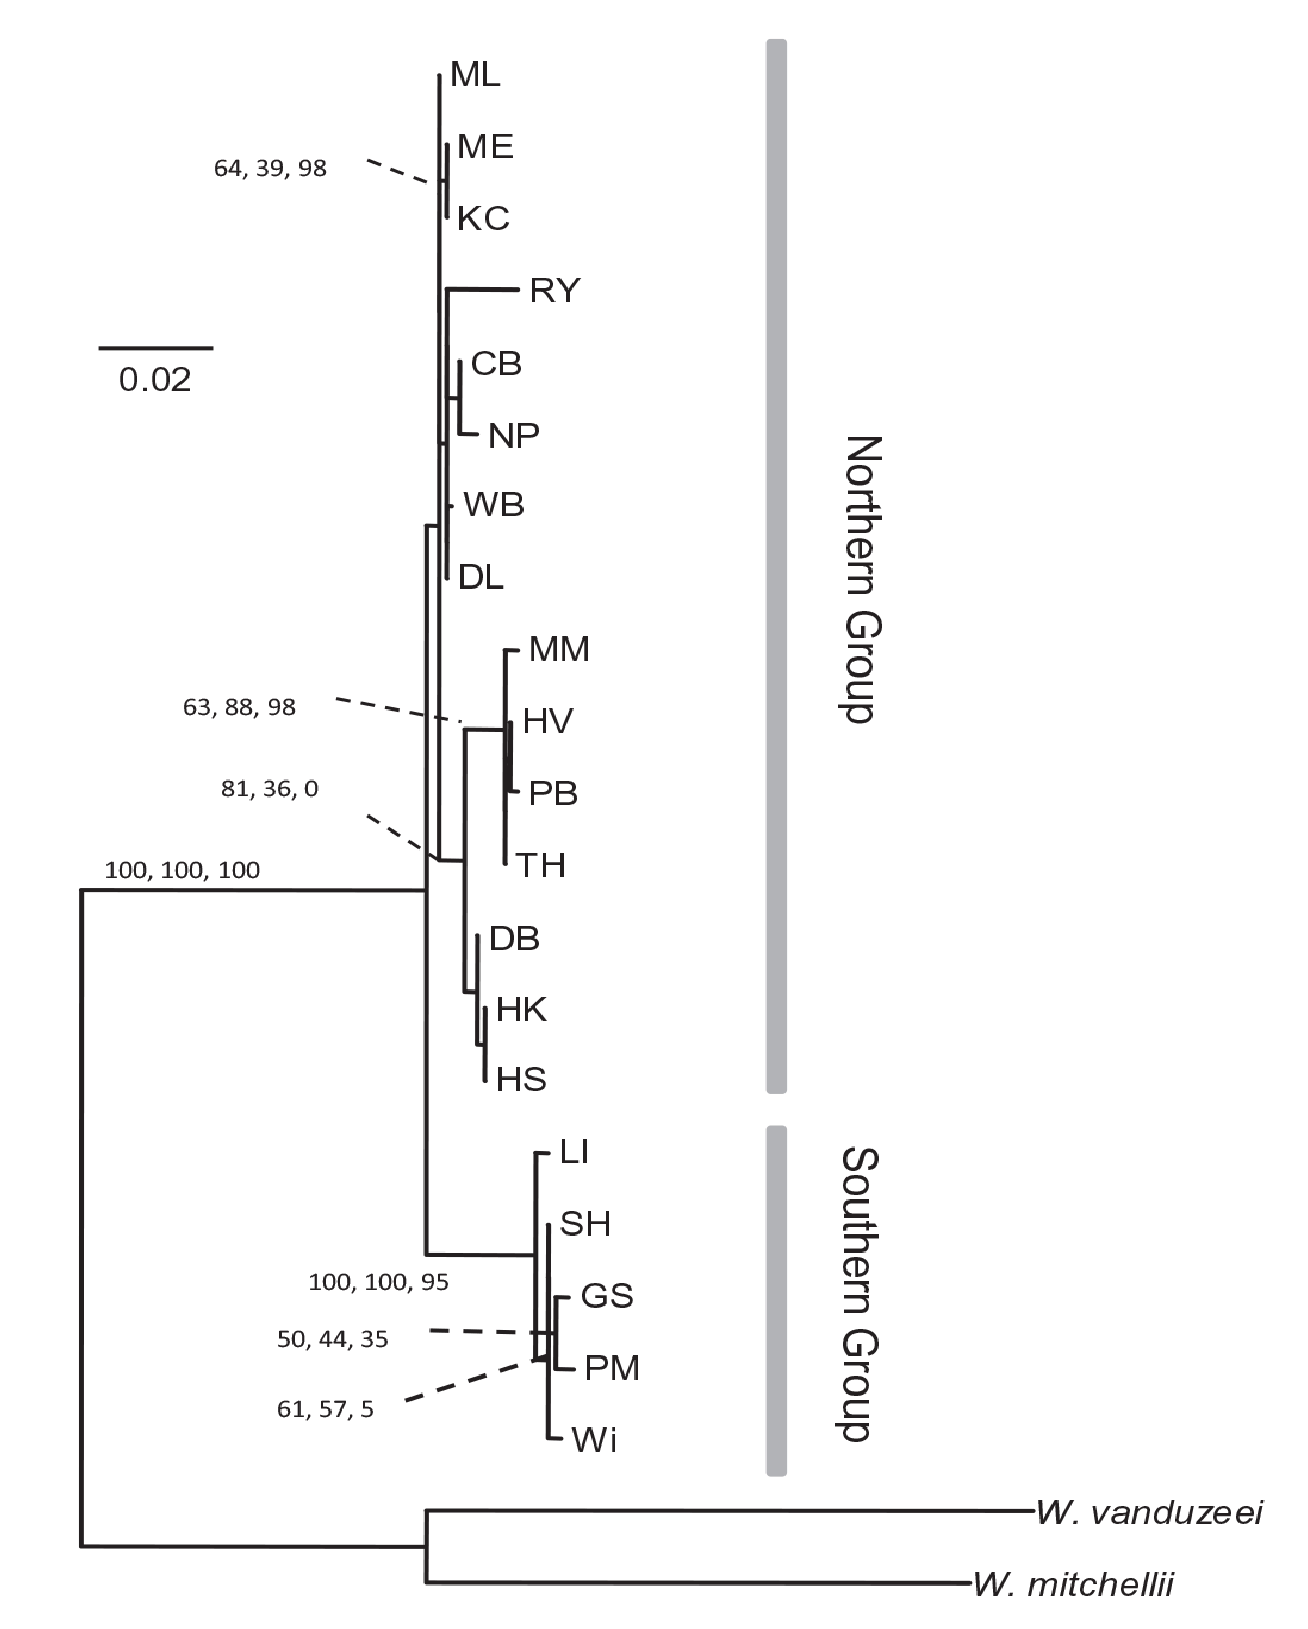
\includegraphics[width=0.9\textwidth]{wyeomyia-COI.eps}
\end{center}
\caption{Maximum-likelihood phylogenetic tree depicting relationshps
  among populations of {\it W. smithii\/} relative to the outgroups
  {\it W. vanduzeei\/} and {\it W. mitchelli} (from~\cite{Emerson-etal-2010}).}\label{fig:wyeomyia-COI}
\end{figure}

Using the same set of samples, the authors used RAD sequencing to
identify 3741 SNPs. That's more than 20 times the number of variable
sites found in {\it COI}, 167. Not surprisingly, the large number of
additional sites allowed the authors to produce a much more highly
resolved phylogeny~(Figure \ref{fig:wyeomyia-RAD}). With this
phylogeny it's easy to see that southern populations are divided into
two distinct groups, those from North Carolina and those from the Gulf
Coast. Similarly, the northern group of populations is subdivided into
those from the Appalachians in North Carolina, those from the
mid-Atlantic coast, and those from further north. The glacial history
of North America means that both the mid-Atlantic populations and the
populations farther north must have been derived from one or more
southern populations after the height of the last glaciation. Given
the phylogenetic relationships recovered here, it seems clear that
they are most closely related to populations in the Appalachians of
North Carolina.

\begin{figure}
\begin{center}
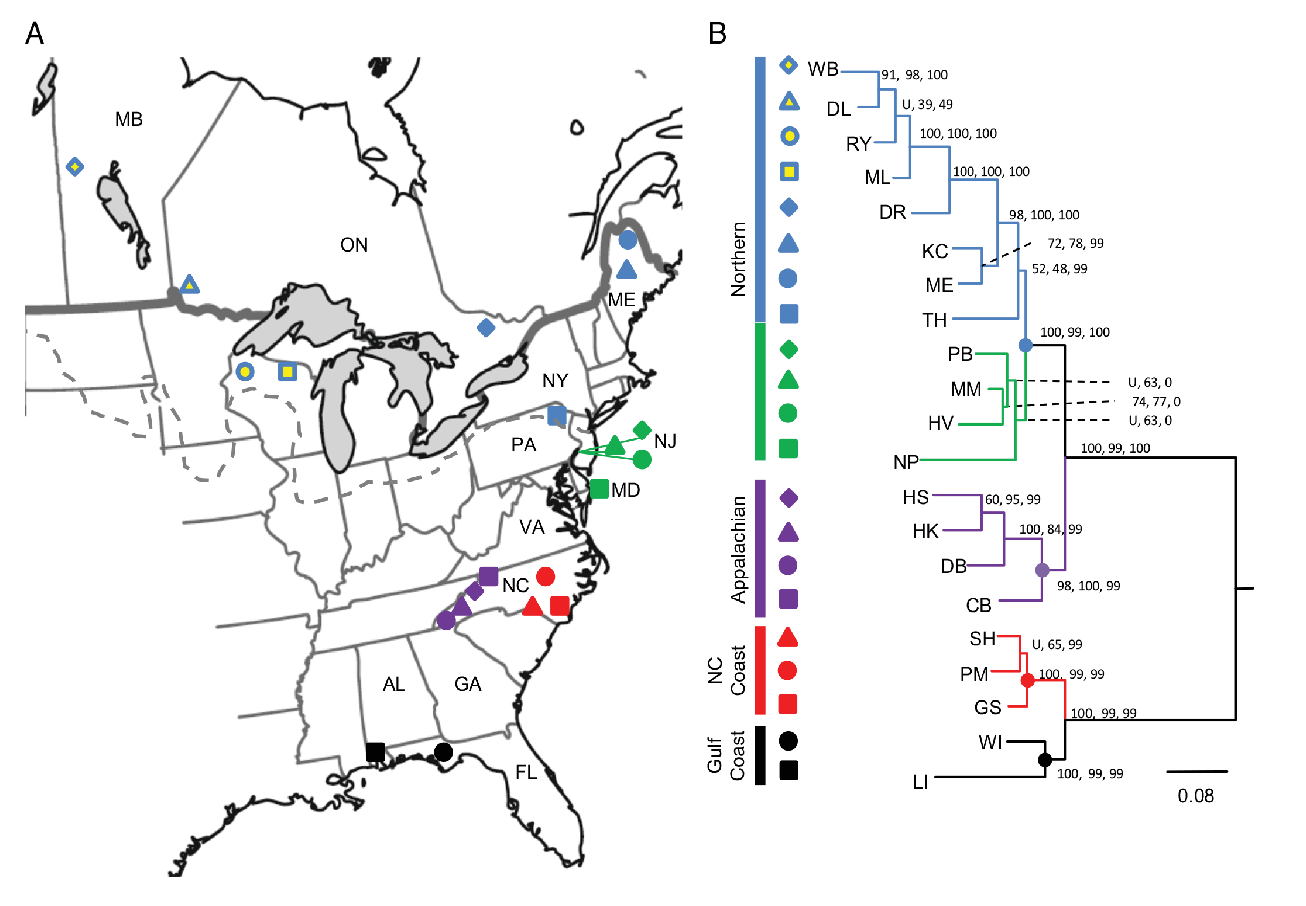
\includegraphics[width=0.9\textwidth]{wyeomyia-RAD.eps}
\end{center}
\caption{A. Geographical distribution of samples included in the
  analysis. B. Phylogenetic relationship of samples included in the analysis.}\label{fig:wyeomyia-RAD}
\end{figure}

That's the promise of NGS for population genetics. What are the
challenges? Funny you should ask.

\section*{Estimates of nucleotide diversity\footnote{This section draws heavily on~\cite{Lynch-2008}}}\index{next-generation sequencing!estimating nucleotide diversity}

Beyond the simple challenge of dealing with all of the short DNA
fragments that emerge from high-throughput sequencing, there are at
least two challenges that don't arise with data obtained in more
traditional ways.

\begin{enumerate}

\item Most studies involve ``shotgun'' sequencing of entire
  genomes. In large diploid genomes, this leads to variable
  coverage. At sites where coverage is low, there's a good chance that
  all of the reads will be derived from only one of the two
  chromosomes present, and a heterozygous individual will be scored as
  homozygous. ``Well,'' you might say, ``let's just throw away all of
  the sites that don't have at least 8$\times$ coverage.''\footnote{If
    both chromosomes have an equal probability of being sequenced, the
    probability that one of them is missed with 8$\times$ coverage is
    $(1/2)^8 = 1/256$.} That would work, but you would also be
  throwing out a lot of potentially valuable information.\footnote{It's
    valuable information, providing you know how to deal with in
    properly.} It seems better to develop an approach that lets us use
  {\it all\/} of the data we collect.

\item Sequencing errors are more common with high-throughput methods
  than with traditional methods, and since so much data is produced,
  it's not feasible to go back and resequence apparent polymorphisms
  to see if they reflect sequencing error rather than real
  differences. Quality scores can be used, but they only reflect the
  quality of the reads from the sequencing reaction, not errors that
  might be introduced during sample preparation. Again, we might focus
  on high-coverage sites and ignore ``polymorphisms'' associated with
  single reads, but we'd be throwing away a lot of
  information.\footnote{To be honest, though, we did ignore a lot of
    data in the analysis of GBS data from {\it Protea repens\/} that
    you may remember from earlier this semester.} 

\end{enumerate}
A better approach than setting arbitrary thresholds and throwing away
data is to develop an explicit model of how errors can arise during
sequencing and to use that model to interpret the data we've
collected. That's precisely the approach that Lynch~\cite{Lynch-2008}
adopts. Here's how it works assuming that we have a sample from a
single, diploid individual:

\begin{itemize}

\item Any particular site will have a sequence profile, $(n_1, n_2,
  n_3, n_4)$, corresponding to the number of times an A, C, G, or T
  was observed. $n=n_1+n_2+n_3+n_4$ is the depth of coverage for that
  site. 

\item Let $\epsilon$ be the probability of a sequencing error at any
  site, and assume that all errors are equiprobable, e.g., there's no
  tendency for an A to be miscalled as a C rather than a T when it's
  miscalled.\footnote{It wouldn't be hard, conceptually, to allow
    different nucleotides to have different error rates, e.g.,
    $\epsilon_A$, $\epsilon_C$, $\epsilon_G$, $\epsilon_T$, but the
    notation would get really complicated, so we won't bother trying
    to show how differential error rates can be accommodated.} 

\item If the site in question were homozygous A, the probability of
  getting our observed sequence profile is:
\[
P(n_1,n_2,n_3,n_4|\mbox{homozygous A},\epsilon)
=
{n \choose n_1}(1-\epsilon)^{n_1}\epsilon^{n-n_1} \quad .
\]
A similar relationship holds if the site were homozygous C, G, or
T. Thus, we can calculate the probability of our data if it were homozygous
as\footnote{This expression
    looks a little different from the one in~\cite{Lynch-2008}, but
    I'm pretty sure it's equivalent.}
\[
P(n_1,n_2,n_3,n_4|\mbox{homozygous},\epsilon)
=
\sum_{i=1}^4 \left(\frac{p_i^2}{\sum_{j=1}^4p_j^2}\right) 
{n \choose n_i}(1-\epsilon)^{n_i}\epsilon^{n-n_i}
\quad .
\]

\item If the site in question were heterozygous, the probability of
  getting our observed sequence profile is a bit more complicated. Let
  $k_1$ be the number of reads from the first chromosome and $k_2$ be
  the number of reads from the second chromosome ($n=k_1+k_2$). Then
\begin{eqnarray*}
P(k_1,k_2)
&=&
{n \choose k_1}\left(\frac{1}{2}\right)^{k_1}
               \left(\frac{1}{2}\right)^{k_2}
\\
&=&
{n \choose k_1}\left(\frac{1}{2}\right)^n \quad .
\end{eqnarray*}
Now consider the ordered genotype $x_ix_j$, where $x_i$ refers to the
nucleotide on the first chromosome and $x_j$ refers to the nucleotide
on the second chromosome. The probability of getting our observed
sequence profile from this genotype given that we have $k_1$ reads
from the first chromosome and $k_2$ reads from the second is:
{\footnotesize
\begin{eqnarray*}
P(n_1,n_2,n_3,n_4|x_i,x_j,k_1,k_2)
&=&
\sum_{l=1}^4\sum_{m=0}^{k_1}{k_1 \choose m}(1-\delta_{il})^m\delta_{il}^{k_1-m}
{k_2 \choose n_i-m}(1-\delta_{jl})^{n_1-m}\delta_{jl}^{k_2-(n_1-m)}
\quad ,
\end{eqnarray*}
}
where 
\[
\delta_{il} = \left\{\begin{array}{ll}
1-\epsilon & \mbox{if } i = l \\
\epsilon & \mbox{if } i \ne l \quad .
\end{array}
\right.
\]
We can use Bayes' Theorem\footnote{Ask me for details if you're
  interested.} to get
\[
P(n_1,n_2,n_3,n_4|x_i,x_j,\epsilon) =
P(n_1,n_2,n_3,n_4|x_i,x_j,k_1,k_2,\epsilon)P(k_1,k_2) \quad ,
\]
and with that in hand we can get
\[
P(n_1,n_2,n_3,n_4|\mbox{heterozygous},\epsilon)
=
\sum_{i=1}^4\sum_{j\ne i}
\left(\frac{x_ix_j}{1-{\sum_{l=1}^4p_l^2}}\right) P(n_1,n_2,n_3,n_4|x_i,x_j,\epsilon) 
\]

\item Let $\pi$ be the probability that any site is heterozygous. Then
  the probability of getting our data is:
{\footnotesize
\[
P(n_1,n_2,n_3,n_4|\pi,\epsilon)
=
\pi P(n_1,n_2,n_3,n_4|\mbox{heterozygous},\epsilon)
+
(1-\pi)P(n_1,n_2,n_3,n_4|\mbox{homozygous},\epsilon) \quad .
\]
}

\item What we've just calculated is the probability of the
  configuration we observed at a particular site. The probability of
  our data is just the product of this probability across all of the
  sites in our sample:
\[
P(\mbox{data}|\pi,\epsilon) = \prod_{s=1}^S
P(n_1^{(s)},n_2^{(s)},n_3^{(s)},n_4^{(s)}|\pi,\epsilon) \quad ,
\]
where the superscript $(s)$ is used to index each site in the data.

\item What we now have is the likelihood of the data in terms of
  $\epsilon$, which isn't very interesting since it's just the average
  sequencing error rate in our sample, and $\pi$, which is
  interesting, because it's the genome-wide nucleotide diversity. Now
  we ``simply'' maximize that likelihood, and we have
  maximum-likelihood estimates of both parameters. Alternatively, we
  could supply priors for $\epsilon$ and $\pi$ and use MCMC to get
  Bayesian estimates of $\epsilon$ and $\pi$.  

\end{itemize}

Notice that this genome-wide estimate of nucleotide diversity is
obtained from a sample derived from a single diploid
individual. Lynch~\cite{Lynch-2008} develops similar methods for
estimating gametic disequilibrium as a function of genetic distance
for a sample from a single diploid individual. He also extends that
method to samples from a pair of individuals, and he describes how to
estimate mutation rates by comparing sequences derived from
individuals in mutation accumulation lines with consensus
sequences.\footnote{Mutation accumulation lines are lines propagated
  through several (sometimes up to hundreds) of generations in which
  population sizes are repeatedly reduced to one or a few individuals,
  allowing drift to dominate the dynamics and alleles to
  ``accumulate'' with little regard to their fitness effects.}

Haubold et al.~\cite{Haubold-etal-2010} describe a program
implementing these methods. Recall that under the infinite sites model
of mutation $\pi = 4N_e\mu$. They analyzed data sets from the sea
squirt {\it Ciona intestinalis\/} and the water flea {\it Daphnia
  pulex}~(Table~\ref{table:NGS-results}). Notice that the sequencing
error rate in {\it D. pulex} is indistinguishable from the nucleotide
diversity.\index{Cionia@\textit{Cionia}!\textit{intestinalis}}\index{Daphnia@\textit{Daphnia}!\textit{pulex}}

\begin{table}
\begin{center}
\begin{tabular}{lccc}
\hline\hline
Taxon & $4N_e\mu$ & $4N_e\mu$ (low coverage) & $\epsilon$ \\
\hline
{\it Cionia intestinalis} & 0.0111 & 0.012 & 0.00113 \\
{\it Daphnia pulex} & 0.0011 & 0.0012 & 0.00121 \\
\hline
\end{tabular}
\end{center}
\caption{Estimates of nucleotide diversity and sequencing error rate
  in {\it Cionia intestinalis\/} and {\it Daphnia pulex}~(results
  from~\cite{Haubold-etal-2010}).}\label{table:NGS-results}
\end{table}

\section*{Next-generation AMOVA\footnote{This section depends heavily on~\cite{Gompert-Buerkle-2011}}}\index{next-generation sequencing!partitioning diversity}\index{BAMOVA}

What we've discussed so far gets us estimates of some population
parameters~($4N_e\mu$, $4N_er$), but they're derived from the
sequences in a single diploid individual. That's not much of a
population sample, and it certainly doesn't tell us anything about how
different populations are from one another. Gompert and
Buerkle~\cite{Gompert-Buerkle-2011} describe an approach to estimate
statistics very similar to $\Phi_{ST}$ from AMOVA. Since they take a
Bayesian approach to developing their estimates, they refer to
approach as BAMOVA, Bayesian models for analysis of molecular
variance. They propose several related models.

\begin{itemize}

\item {\bf NGS-individual model}: This model assumes that sequencing
  errors are negligible.\footnote{Or that they've already been
    corrected. We don't care {\it how\/} they might have been
    corrected. We care only that we can assume that the reads we get
    from a sequencing run faithfully reflect the sequences present on
    each of the chromosomes.} Under this model, the only trick is that
  we may or may not pick up both sequences from a heterozygote. The
  probability of not seeing both sequences in a heterozygote is
  related to the depth of coverage.

\item {\bf NGS-population model}: In some NGS experiments,
  investigators pool all of the samples from a population into a
  single sample. Again, Gompert and Buerkle assume that sequencing
  errors are negligible. Here we assume that the number of reads for
  one of two alleles at a particular SNP site in a sample is related
  to the underlying allele frequency at that site. Roughly speaking,
  the likelihood of the data at that site is then
\[
P(x_i|p_i,n_i, k_i) = {n_i \choose k_i}p_i^{k_i}(1-p_{i})^{n-k_i}
\quad ,
\]
where $p_i$ is the allele frequency at this site, $n_i$ is the sample
size, and $k_i$ is the count of one of the alleles in the sample. The
likelihood of the data is just the product across the site-specific
likelihoods.\footnote{The actual model they use is a bit more
  complicated than this, but the principles are the same.}

\end{itemize}

Then, as we did way back when we used a Bayesian appraach to estimate
$F_{ST}$~\cite{Holsinger-Wallace-2004}, we put a prior on the $p_i$
and the parameters of this prior are defined in terms of
$\Phi_{ST}$~(among other things).\footnote{Again, the actual model is
  a bit more complicated than what I'm describing here, but the
  principle is the same.} They also propose a method for detecting SNP
loci\footnote{Or sets of SNP loci that are parts of a single contig.}
that have unusually large or small values of $\Phi_{ST}$.

\subsection*{BAMOVA example}\index{BAMOVA!example}

Gompert and Buerkle~\cite{Gompert-Buerkle-2011} used data derived from
two different human population data sets:

\begin{itemize}

\item 316 fully sequenced genes in an African population and a
  population with European ancestry. With these data, they didn't have
  to worry about the sequencing errors that their model neglects and
  they could simulate pooled samples allowing them to compare
  estimates derived from pooled versus individual-level data.

\item 12,649 haplotype regions and 11,866 genes derived from 597
  individuals across 33 widely distributed human populations.

\end{itemize}

In analysis of the first data set, they estimated
$\Phi_{ST}=0.08$. Three loci were identified as having unusually high
values of $\Phi_{ST}$. 

\begin{itemize}

\item {\bf HSD11B2}: $\Phi_{ST}=0.32 (0.16,0.48)$. Variants at this
  locus are associated with an inherited form of high blood pressure
  and renal disease. A microsatellite in an intron of this locus is
  weakly associated with type 1 diabetes.

\item {\bf FOXA2}: $\Phi_{ST}=0.32 (0.12,0.51)$. This gene is involved
  in reguation of insulin sensitivity.

\item {\bf POLG2}: $\Phi_{ST}=0.33 (0.18,0.48)$. This locus was
  identified as a target of selection in another study.

\end{itemize}

In analysis of the 33-population data set, they found similar values
of $\Phi_{ST}$ on each chromosome, ranging from 0.083 (0.075, 0.091)
on chromosome 22 to 0.11 (0.10, 0.12) on chromosome 16. $\Phi_{ST}$
for the X chromosome was marginally higher: 0.14 (0.13,0.15). They
detected 569 outlier loci, 518 were high outliers and 51 were low
outliers. Several of the loci they detected as outliers had been
previously identified as targets of selection. The loci they
identified as candidates for balancing selection have not been
suggested before as targets of such selection.

\section*{Estimating population structure}

In addition to $F_{ST}$ we saw that a principal components analysis of
genetic data might sometimes be useful. Fumagalli et
al.~\cite{Fumagalli-etal-2013} develop a method for PCA that, like
Lynch's~\cite{Lynch-2008} method for estimating nucleotide diversity,
uses all of the information available in NGS data rather than imposing
an artificial threshold for calling genotypes. They calculate the
pairwise entries of the covariance matrix by integrating across the
genotype probabiity at each site as part of the calculation and
weighting the contribution of each site to the analysis by the
probability that it is
variable.\footnote{See~\cite{Fumagalli-etal-2013} for details.} As
shown in Figure~\ref{fig:Fumagalli-PCA} this approach to PCA recovers
the structure much better than approaches that simply call genotypes
at each locus, whether or not outliers are excluded. The authors also
describe approaches to estimating $F_{ST}$ that take account of the
characteristics of NGS data. Their software ({\tt ANGSD}:
\url{http://popgen.dk/wiki/index.php/ANGSD}) implements these and
other useful statistical analysis tools for next-generation sequencing
data, including Tajima's D. They also provide {\tt NgsAdmix} for {\tt
  Structure}-like analyses of NGS
data~(\url{http://www.popgen.dk/software/index.php/NgsAdmix}). 

\begin{figure}
\begin{center}
\includegraphics[width=10cm]{fumagalli-PCA.eps}
\end{center}
\caption{The ``true genotypes'' PCA is based on the actual, simulated
  genotypes (20 individuals in each population, 10,000 sites in the
  sample with 10\% variable; $F_{ST}$ between the purple population
  and either the red or the green population was 0.4 and between the
  green and red populations was 0.15; and coverage was simulated at
  $2\times$~(from~\cite{Fumagalli-etal-2013}).}\label{fig:Fumagalli-PCA}
\end{figure}

\section*{Genetic structure of human populations in Great Britain}

As we've seen several times in this course, the amount of genetic data
available on humans is vastly greater than what is available for any
other organism. As a result, it's possible to use these data to gain
unusually deep insight into the recent history of many human
populations. Today's example comes from Great Britain, courtesy of a
very large consortium~\cite{Leslie-etal-2015}

\subsection*{Data}

\begin{itemize}

\item 2039 individuals with four grandparents born within 80km of one
  another, effectively studying alleles sampled from grandparents
  (ca. 1885). 

\item 6209 samples from 10 countries in continental Europe.

\item Autosomal SNPs genotyped in both samples~(ca. 500K). 

\end{itemize}

\subsection*{Results}

Very little evidence of population structure within British sample

\begin{itemize}

\item Average pairwise $F_{ST}$: 0.0007

\item Maximum pairwise $F_{ST}$: 0.003

\end{itemize}

Individual assignment analysis of genotypes used {\tt fineSTRUCTURE},
which uses the same principle as {\tt STRUCTURE} but models the
correlations among SNPs resulting from gametic disequilibrium, rather
than treating each locus as being independently inherited. The
analysis is on {\it haplotypes\/} rather than on alleles. In addition,
it clusters populations
hierarchically~(Figure~\ref{fig:fine-structure}\index{fineSTRUCTURE}\index{human
  population genetics}

\begin{figure}
\begin{center}
\includegraphics[height=0.9\textheight]{fine-structure-britain.eps}
\end{center}
\caption{{\tt fineSTRUCTURE} analysis of genotypes from Great Britain~(from~\cite{Leslie-etal-2015}).}
\end{figure}

Analysis of the European data identifies 52 groups. The authors used
{\tt Chromopainter} to construct each of the haplotypes detected in
their sample of 2039 individuals from the UK as a mosaic of haplotypes
derived from those found in their sample of 6209 individuals from
continental Europe. Since they know (a) the UK cluster to which each
UK individual belongs and (b) the European group from which each
individual contributing to the UK mosaic belongs they can estimate (c)
the proportion of ancestry for each UK cluster derived from each
European group. The results are shown in Figure~\ref{fig:UK-Europe}.

\begin{figure}
\begin{center}
\includegraphics[width=0.9\textwidth]{UK-Europe.eps}
\end{center}
\caption{European ancestry of the 17 clusters identified in the UK~(from~\cite{Leslie-etal-2015}).}\label{fig:UK-Europe}
\end{figure}

\bibliography{popgen}
\bibliographystyle{plain}

\ccLicense

\end{document}
